%!TEX root = ../../main.tex


\begin{figure}[!htb]
\centering
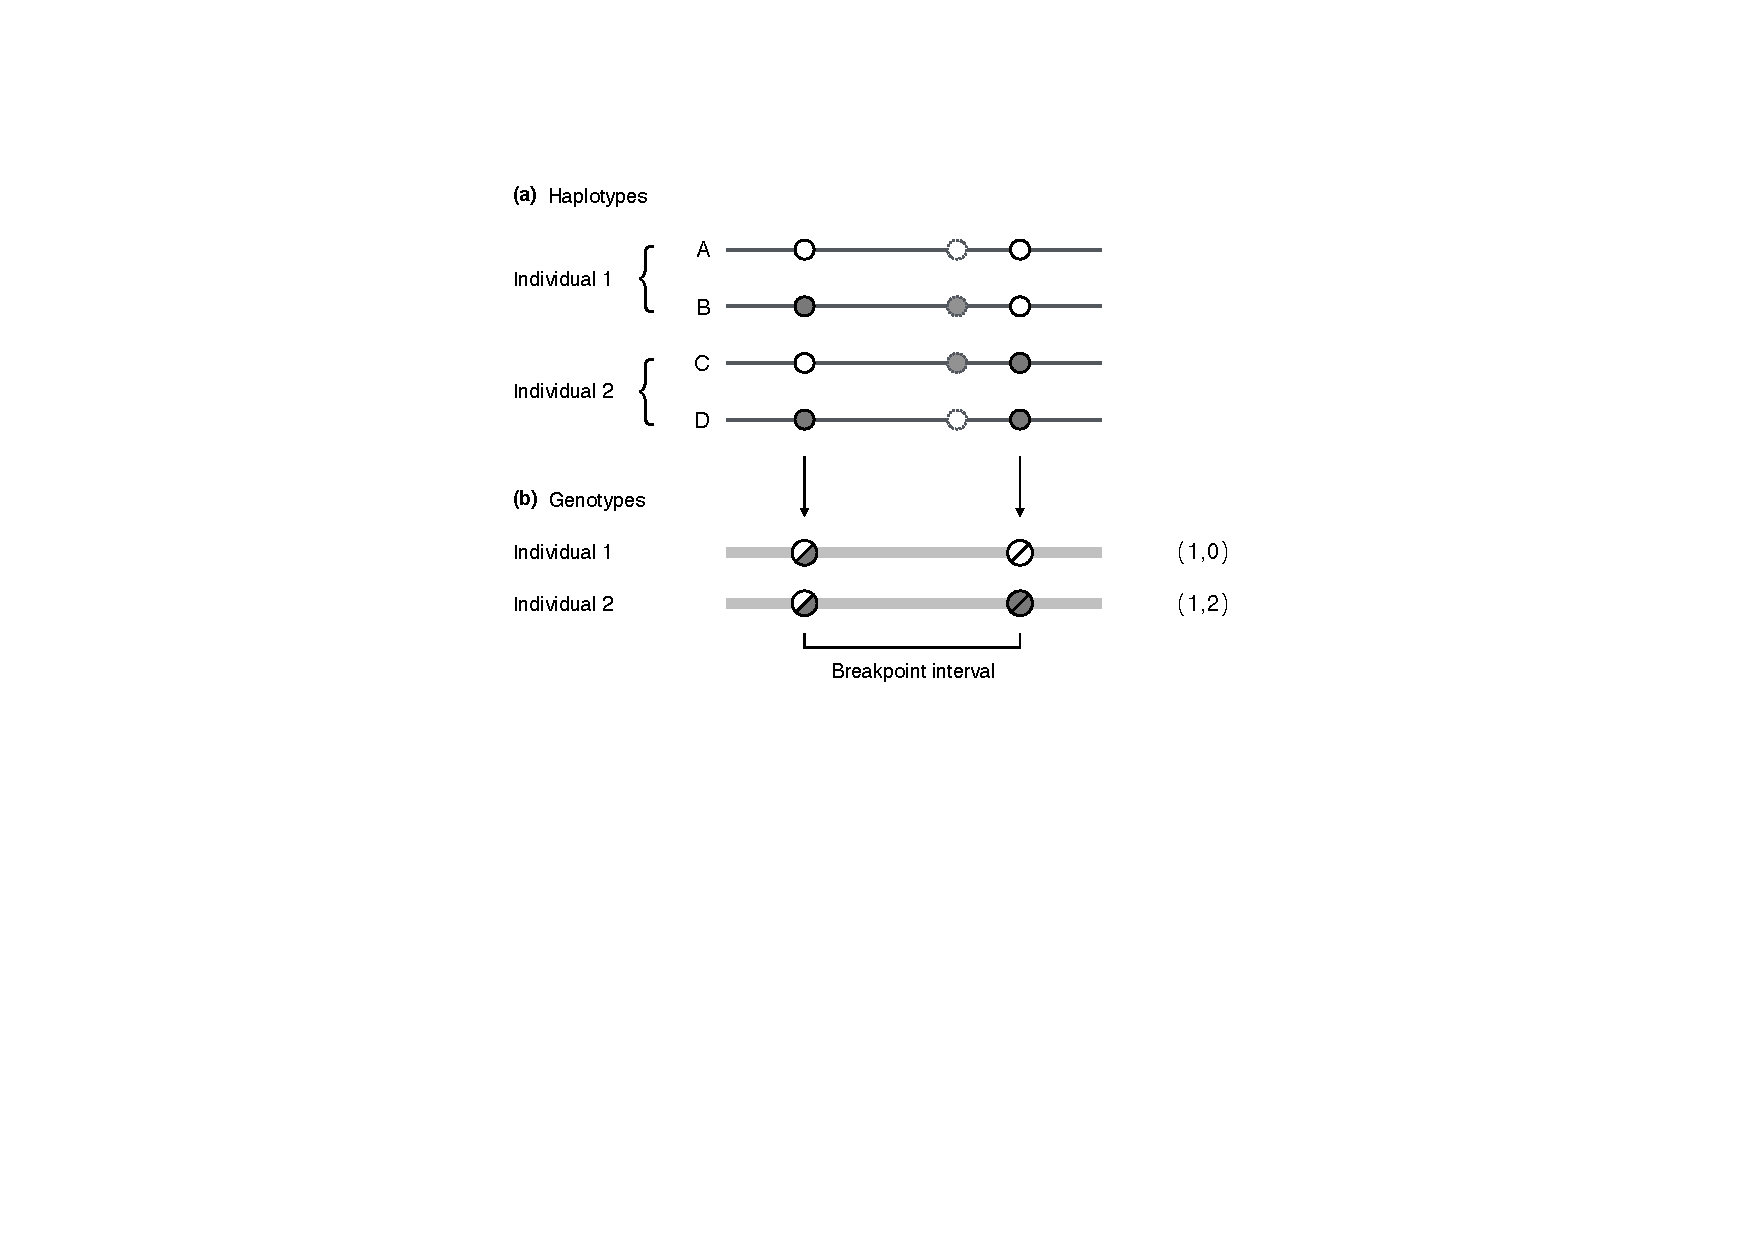
\includegraphics[width=0.7\textwidth]{./img/ch3/info_dgt}
\Caption{Breakpoint detection using the discordant genotype test (DGT)}
{Unlike the \gls{fgt}, which requires haplotype information, the \gls{dgt} identifies a breakpoint interval using genotype data.
For comparison, Panel~\textbf{(a)} shows the \n{4} gametes of the \n{2} individuals involved; see \cpref{fig:info_fgt}.
To highlight the difference to the \gls{fgt}, an additional variant is shown in between both sites; alleles indicated by a \emph{dotted} edge.
This site would satisfy the breakpoint condition under the \gls{fgt}, but is missed under the \gls{dgt}.
Panel~\textbf{(b)} shows the \n{2} genotype sequences per individual (\emph{thick} horizontal lines) from which a breakpoint interval is inferred using the \gls{dgt}.
The genotypic states of the breakpoint sites are given on the \emph{right}.
Genotypes can either be homozygous for the ancestral allele (\emph{hollow} circle), heterozygous (\emph{semi-solid}), or homozygous for the derived allele (\emph{solid}).}
{fig:info_dgt}
\end{figure}
